\documentclass{article}

\usepackage{polski}
\usepackage[utf8]{inputenc}
\usepackage{graphicx}
\usepackage{float}
\usepackage{amsmath}
\usepackage{geometry} 

\author{Jakub Postępski}
\title{MODI, projekt 2, zadanie 33}
\begin{document}
\maketitle
\section{Identyfikacja modeli statycznych}
Wykorzystano dane statyczne dla zestawu 33 (rysunek \ref{fig:danestatyczne}).
\begin{figure}
\centering
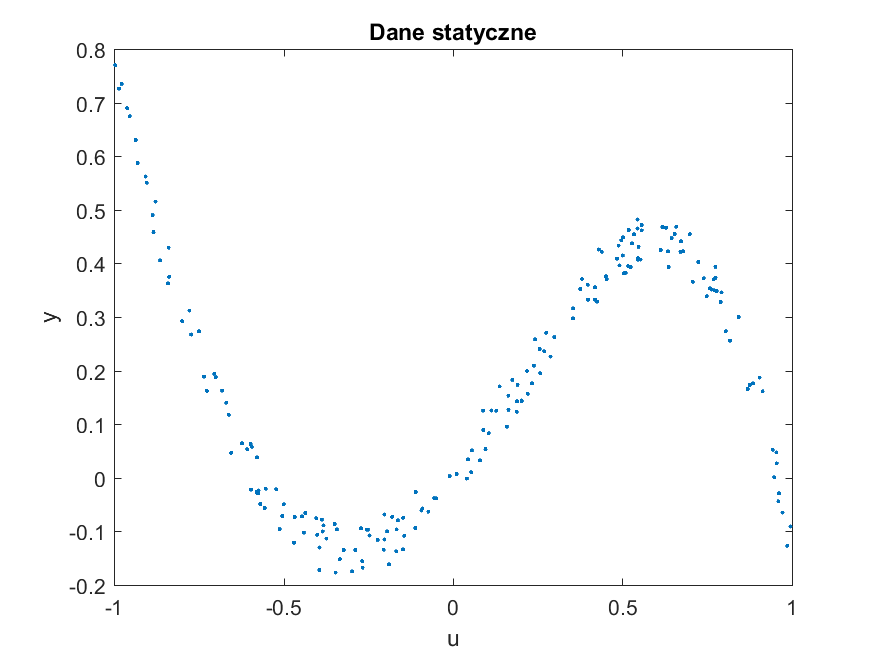
\includegraphics[width=0.95\linewidth]{../dane_statyczne/dane_statyczne}
\caption{Dane statyczne}
\label{fig:danestatyczne}
\end{figure}

Podzielono dane statyczne na zbiór uczący (rysunek \ref{fig:danestatyczneuczace}) oraz zbiór weryfikujący (rysunek \ref{fig:danestatyczneweryf}), poprzez przypisanie każdego kolejnego elementu danych statycznych do innego zbioru.\\
Wyznaczono statyczne modele nieliniowe postaci
\[y(u) = \sum_{i = 0}^{N}a_i u^i\]

\begin{tabular}{|c|c|c|c|c|c|c|c|c|c|}
\hline 
$N$ & $a_0$ & $a_1$ & $a_2$ & $a_3$ & $a_4$ & $a_5$ & $a_6$ & $E_{ucz}$ & $E_{wer}$ \\ 
\hline 
1 & 0.1806 & 0.0519 & - & - & - & - & - & 0.12872 & 0.0021702 \\ 
\hline 
2 & 0.0447 & 0.0517 & 0.4014 & - & - & - & - & 0.37595 & 0.024406 \\ 
\hline 
3 & 0.0467 &  0.7964&0.3795  &-1.2511  & - & - &-  &0.016417  &0.00019188  \\ 
\hline 
4 & -0.0048 & 0.7935 & 0.8324 & -1.2540  & -0.5050 & - & - & 0.0011411 & 0.00012017 \\ 
\hline 
5 &-0.0049  & 0.8033 & 0.8340 &   -1.2987&  -0.5066& 0.0389 & - & 0.0013553 & 8.5264e-05 \\ 
\hline 
6 & -0.0033 &  0.8037&  0.8039& -1.3017 &-0.4171  &0.0418  & -0.0645 & 0.0012089 & 8.4509e-05 \\ 
\hline 

\end{tabular} 
Należy zaznaczyć, że w tabelce opisany jest też model rzędu pierwszego, czyli model liniowy, z podpunktu c).\\
Według autora najlepszym wyborem jest model z wielomianem stopnia 4. Nie ma on wiele większych błędów niż inne modele i jest stosunkowo prosty.
\begin{figure}
\centering
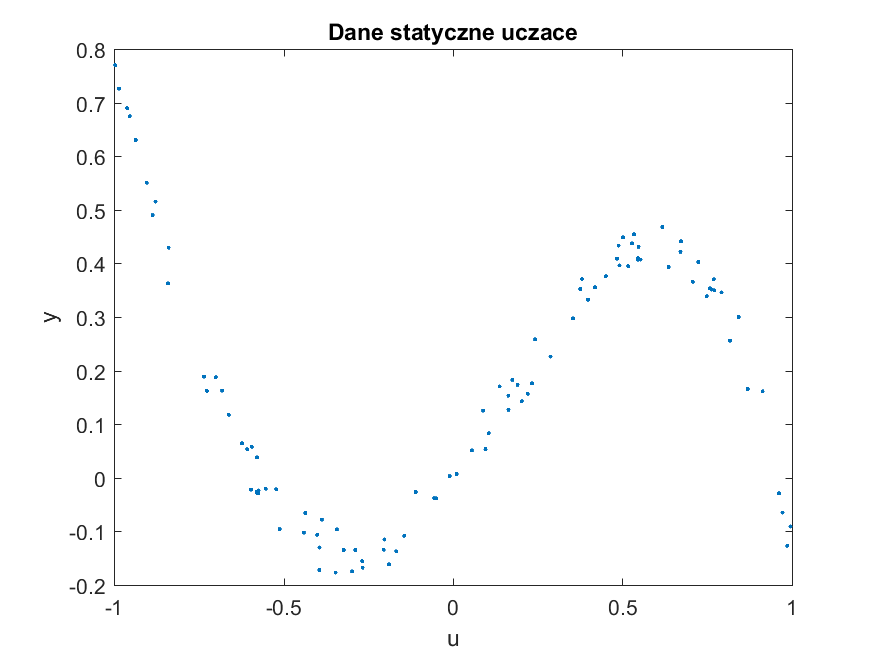
\includegraphics[width=0.95\linewidth]{../dane_statyczne/dane_statyczne_uczace}
\caption{Dane statyczne, zbiór uczący}
\label{fig:danestatyczneuczace}
\end{figure}

\begin{figure}
\centering
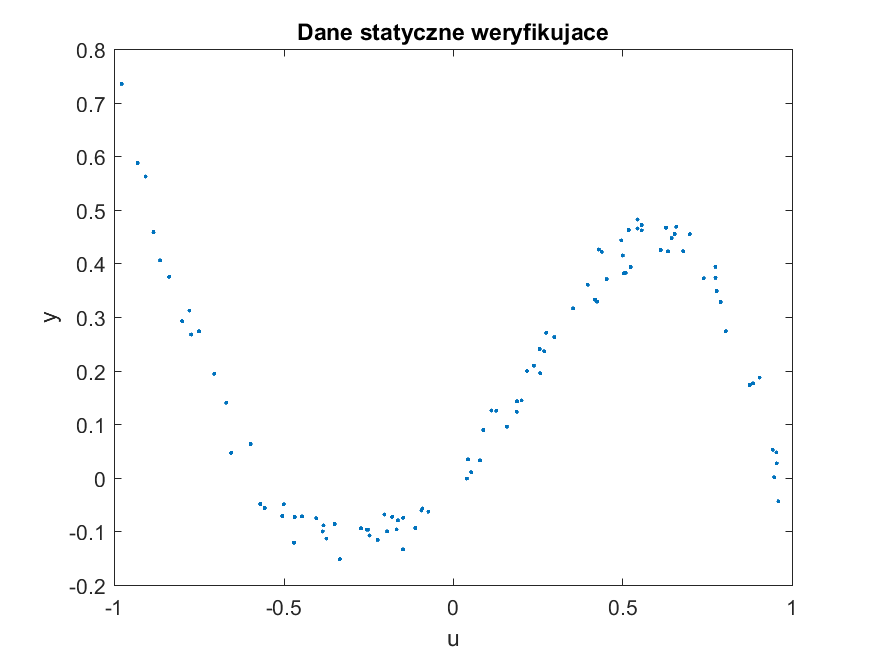
\includegraphics[width=0.95\linewidth]{../dane_statyczne/dane_statyczne_weryf}
\caption{Dane statyczne, zbiór weryfikujący}
\label{fig:danestatyczneweryf}
\end{figure}

\begin{figure}
\centering
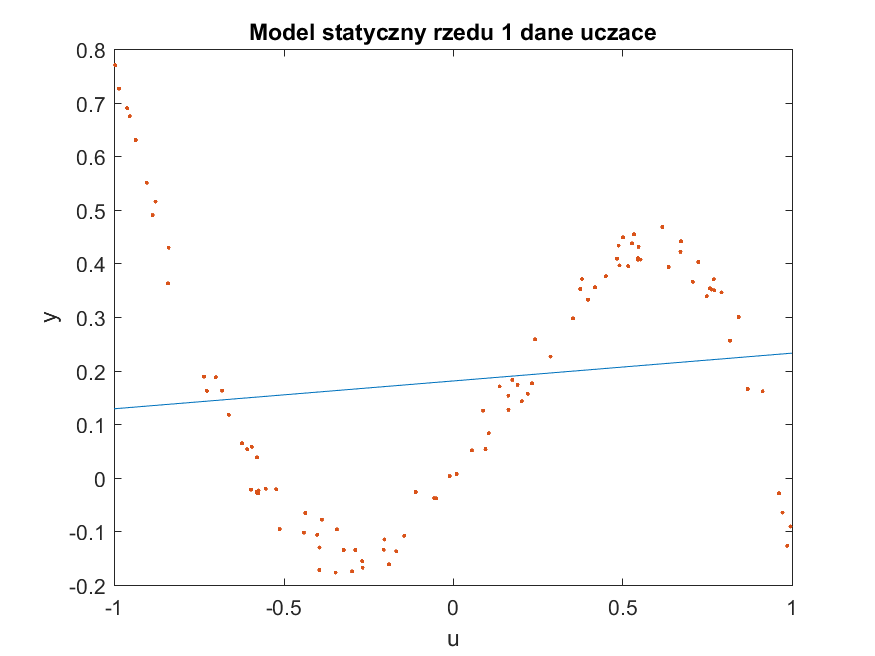
\includegraphics[width=0.95\linewidth]{../dane_statyczne/dane_statyczne_model_rzedu_1_uczace}
\caption{Dane statyczne(uczące) i model dla wielomianu stopnia 1}
\label{fig:danestatyczneuczace1}
\end{figure}

\begin{figure}
\centering
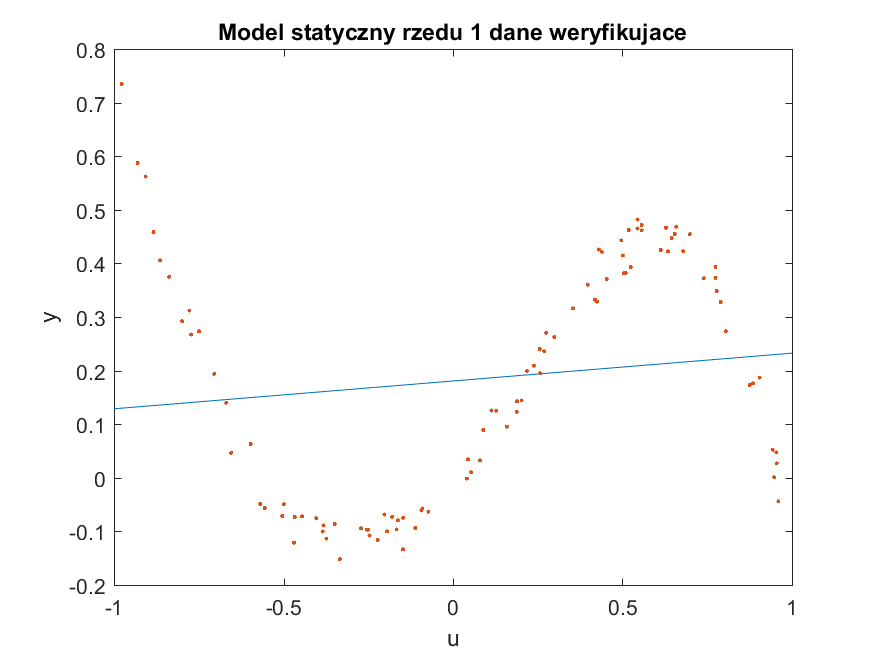
\includegraphics[width=0.95\linewidth]{../dane_statyczne/dane_statyczne_model_rzedu_1_weryf}
\caption{Dane statyczne(weryfikujące) i model dla wielomianu stopnia 1}
\label{fig:danestatyczneweryf1}
\end{figure}

\begin{figure}
\centering
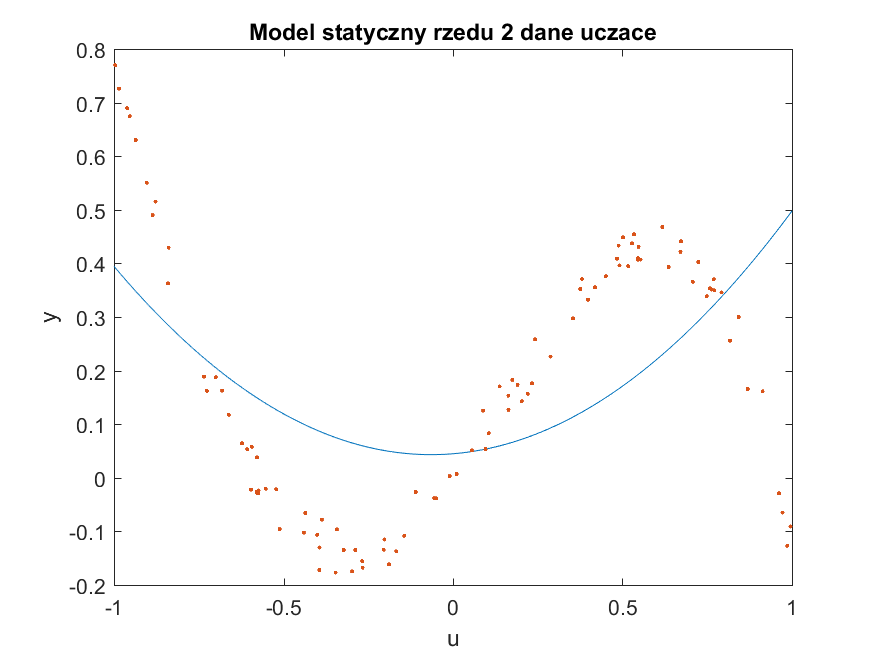
\includegraphics[width=0.95\linewidth]{../dane_statyczne/dane_statyczne_model_rzedu_2_uczace}
\caption{Dane statyczne(uczące) i model dla wielomianu stopnia 2}
\label{fig:danestatyczneuczace2}
\end{figure}

\begin{figure}
\centering
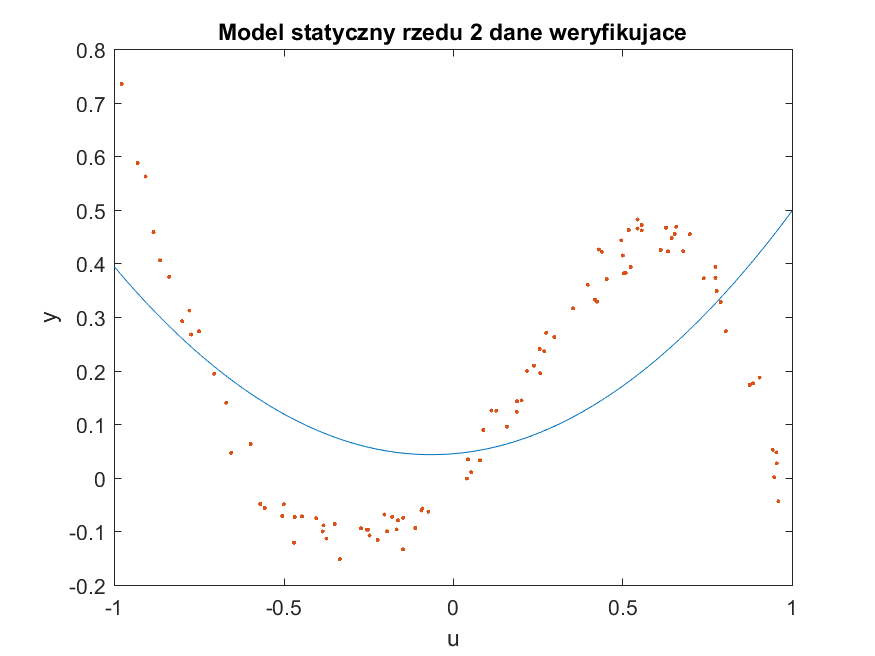
\includegraphics[width=0.95\linewidth]{../dane_statyczne/dane_statyczne_model_rzedu_2_weryf}
\caption{Dane statyczne(weryfikujące) i model dla wielomianu stopnia 2}
\label{fig:danestatyczneweryf2}
\end{figure}

\begin{figure}
\centering
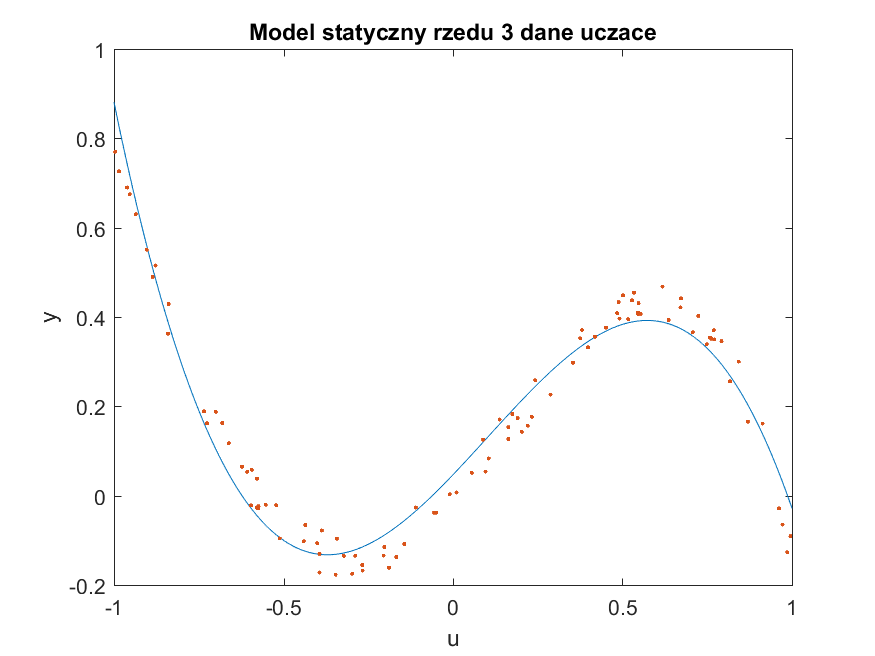
\includegraphics[width=0.95\linewidth]{../dane_statyczne/dane_statyczne_model_rzedu_3_uczace}
\caption{Dane statyczne(uczące) i model dla wielomianu stopnia 3}
\label{fig:danestatyczneuczace3}
\end{figure}

\begin{figure}
\centering
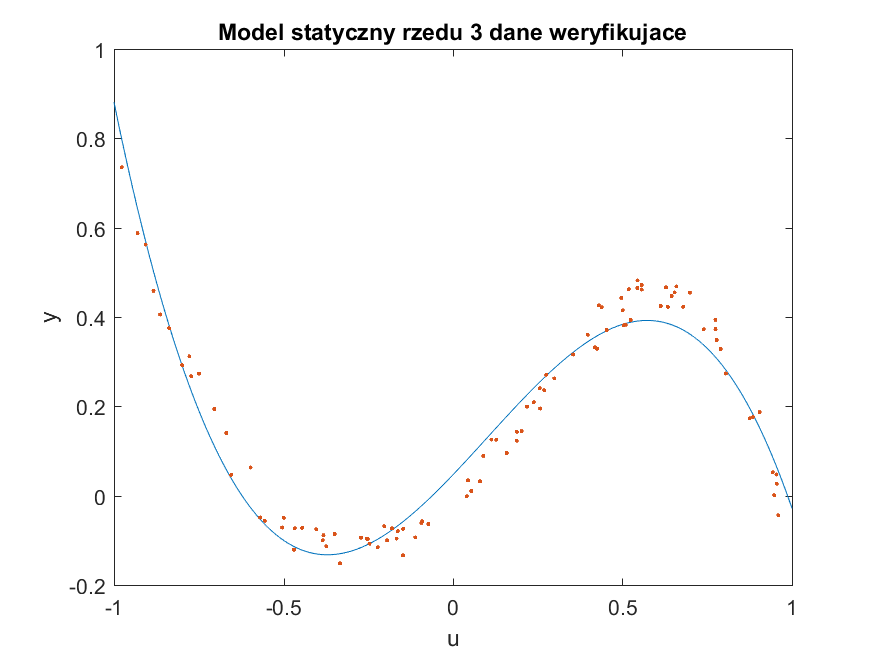
\includegraphics[width=0.95\linewidth]{../dane_statyczne/dane_statyczne_model_rzedu_3_weryf}
\caption{Dane statyczne(weryfikujące) i model dla wielomianu stopnia 3}
\label{fig:danestatyczneweryf3}
\end{figure}

\begin{figure}
\centering
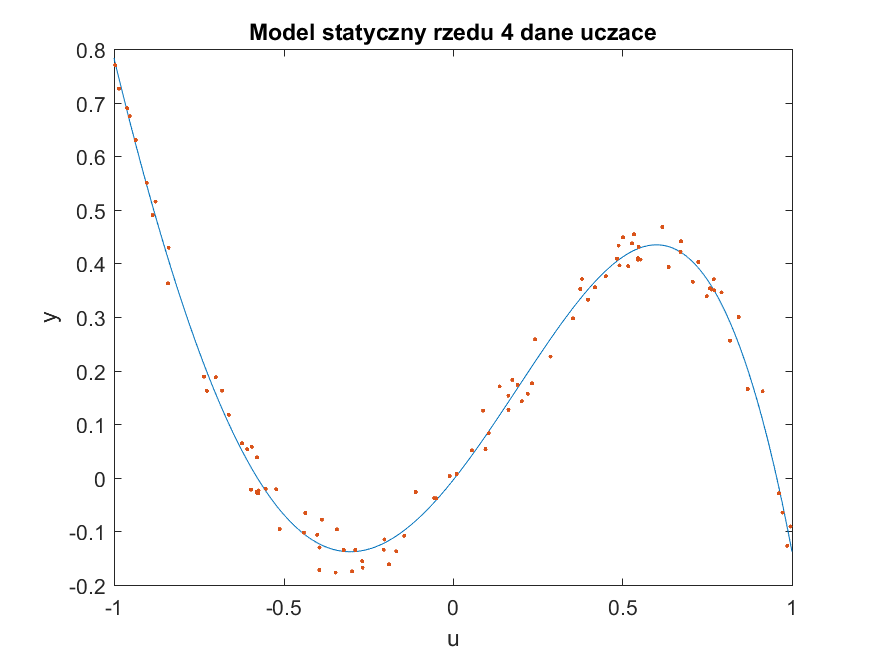
\includegraphics[width=0.95\linewidth]{../dane_statyczne/dane_statyczne_model_rzedu_4_uczace}
\caption{Dane statyczne(uczące) i model dla wielomianu stopnia 4}
\label{fig:danestatyczneuczace4}
\end{figure}

\begin{figure}
\centering
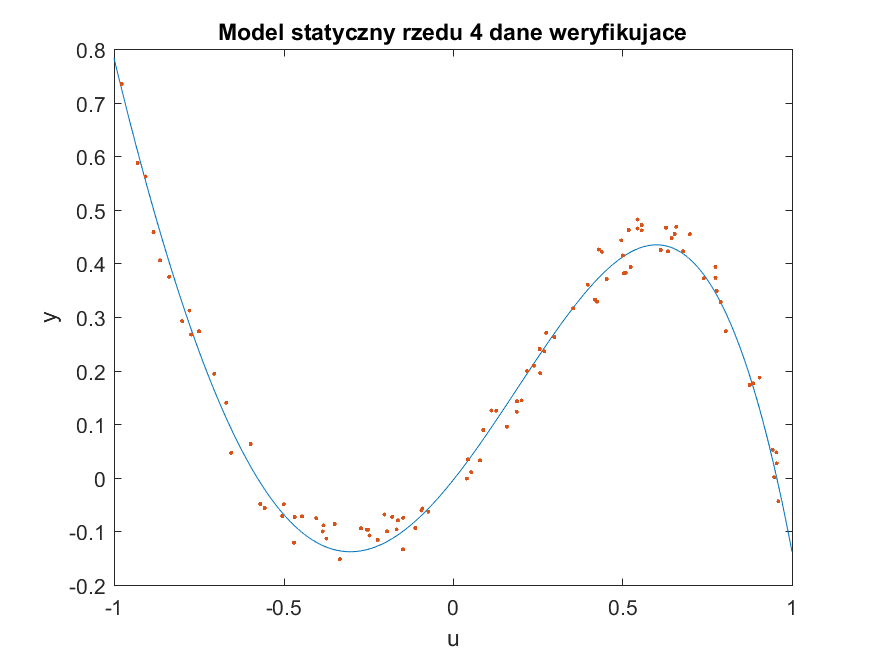
\includegraphics[width=0.95\linewidth]{../dane_statyczne/dane_statyczne_model_rzedu_4_weryf}
\caption{Dane statyczne(weryfikujące) i model dla wielomianu stopnia 4}
\label{fig:danestatyczneweryf4}
\end{figure}

\begin{figure}
\centering
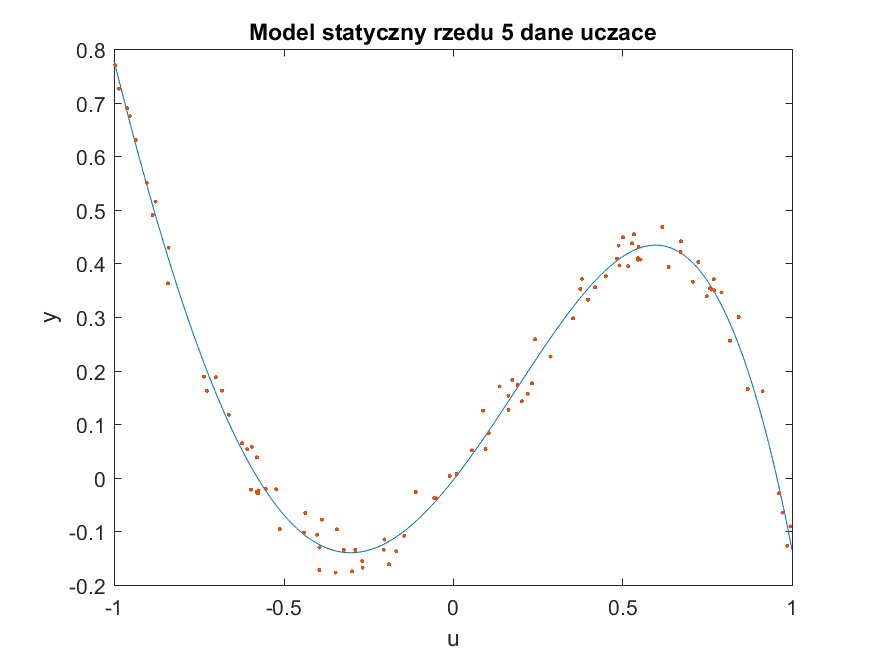
\includegraphics[width=0.95\linewidth]{../dane_statyczne/dane_statyczne_model_rzedu_5_uczace}
\caption{Dane statyczne(uczące) i model dla wielomianu stopnia 5}
\label{fig:danestatyczneuczace5}
\end{figure}

\begin{figure}
\centering
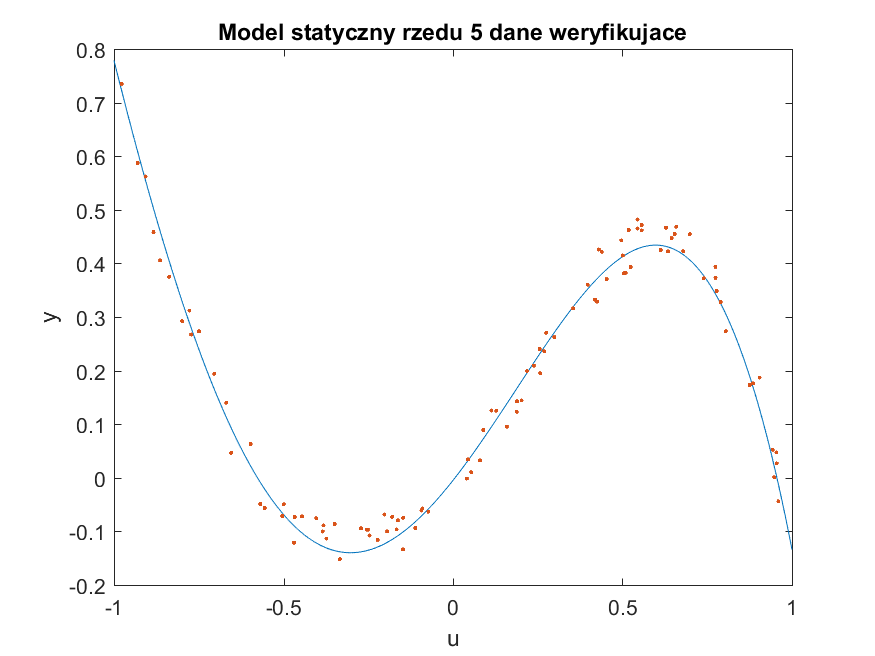
\includegraphics[width=0.95\linewidth]{../dane_statyczne/dane_statyczne_model_rzedu_5_weryf}
\caption{Dane statyczne(weryfikujące) i model dla wielomianu stopnia 5}
\label{fig:danestatyczneweryf5}
\end{figure}

\begin{figure}
\centering
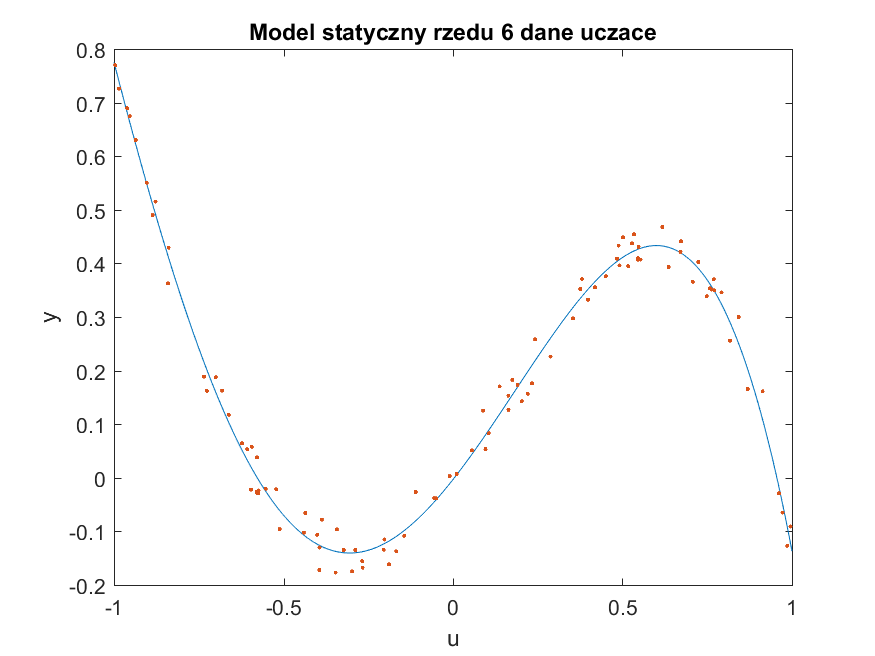
\includegraphics[width=0.95\linewidth]{../dane_statyczne/dane_statyczne_model_rzedu_6_uczace}
\caption{Dane statyczne(uczące) i model dla wielomianu stopnia 6}
\label{fig:danestatyczneuczace3}
\end{figure}

\begin{figure}
\centering
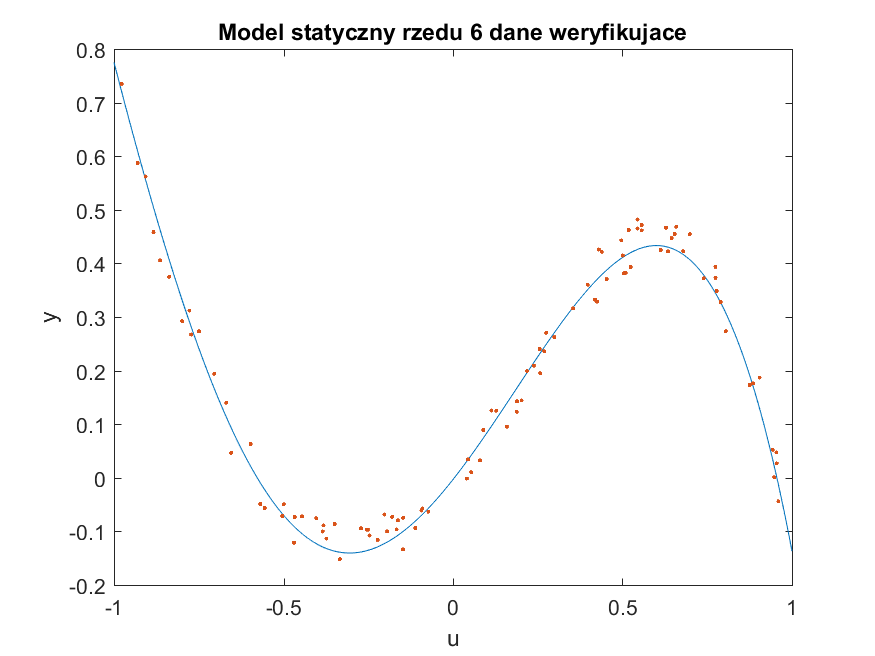
\includegraphics[width=0.95\linewidth]{../dane_statyczne/dane_statyczne_model_rzedu_6_weryf}
\caption{Dane statyczne(weryfikujące) i model dla wielomianu stopnia 6}
\label{fig:danestatyczneweryf6}
\end{figure}
\section{Identyfikacja modeli dynamicznych}
Modele wykonano dla danych uczacych (rysunek \ref{fig:dane_dyn_ucz_u} i \ref{fig:dane_dyn_ucz_y}) i przy pomocy danych weryfikacyjnych (rysunek \ref{fig:dane_dyn_wer_u} i \ref{fig:dane_dyn_wer_y}) walidowano. 

\begin{figure}
\centering
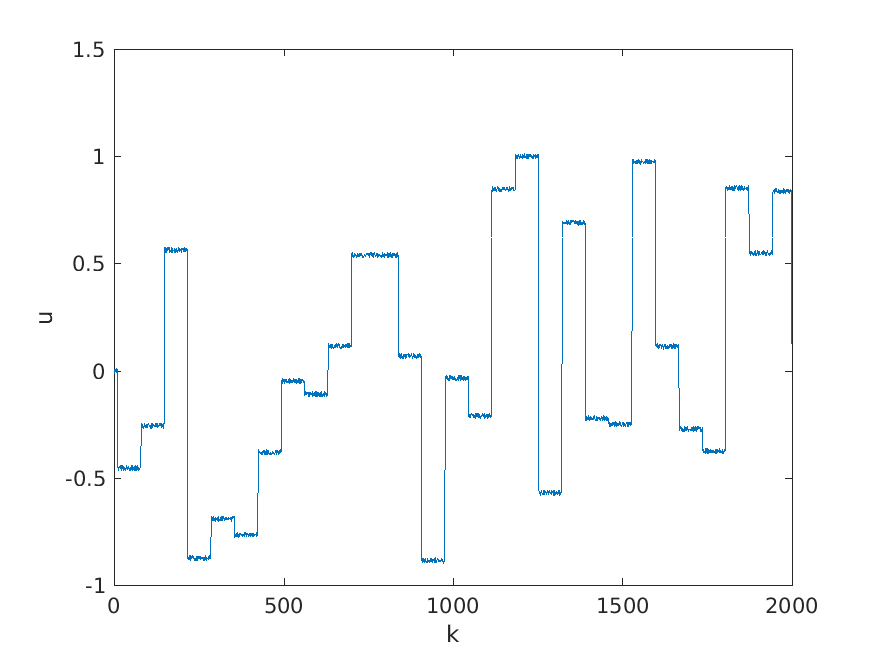
\includegraphics[width=0.7\linewidth]{../dane_dynamiczne/dane_dyn_ucz_u}
\caption{Dane dynamiczne uczące, wejście modelu.}
\label{fig:dane_dyn_ucz_u}
\end{figure}

\begin{figure}
	\centering
	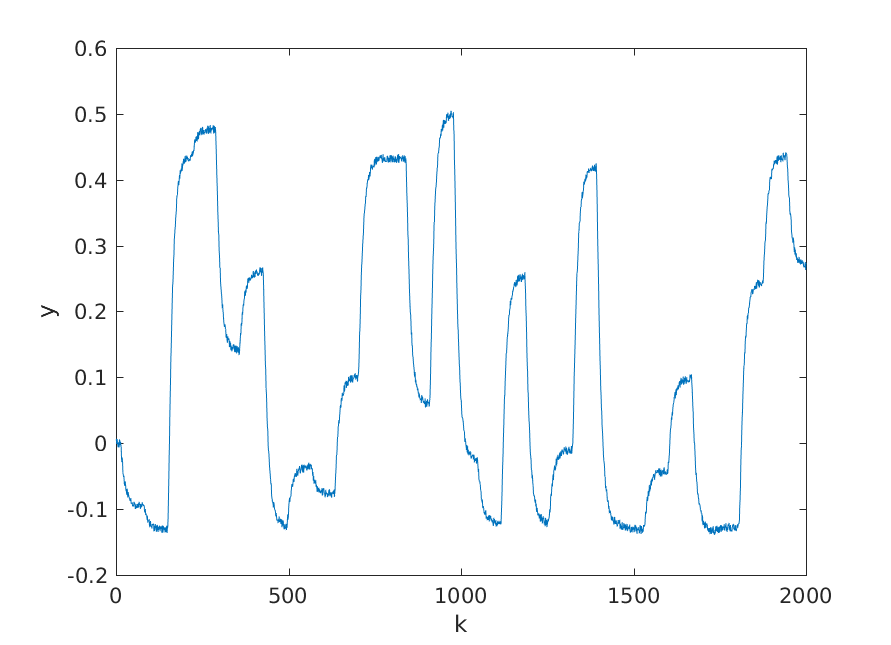
\includegraphics[width=0.7\linewidth]{../dane_dynamiczne/dane_dyn_ucz_y}
	\caption{Dane dynamiczne uczące, wyjście modelu.}
	\label{fig:dane_dyn_ucz_y}
\end{figure}

\begin{figure}
	\centering
	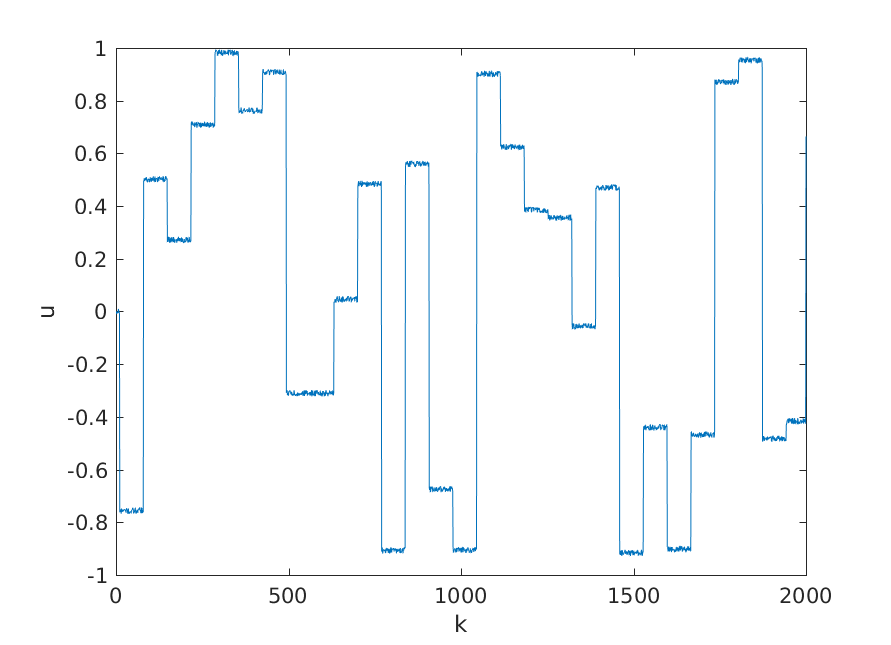
\includegraphics[width=0.7\linewidth]{../dane_dynamiczne/dane_dyn_wer_u}
	\caption{Dane dynamiczne walidujące, wejście modelu.}
	\label{fig:dane_dyn_wer_u}
\end{figure}

\begin{figure}
	\centering
	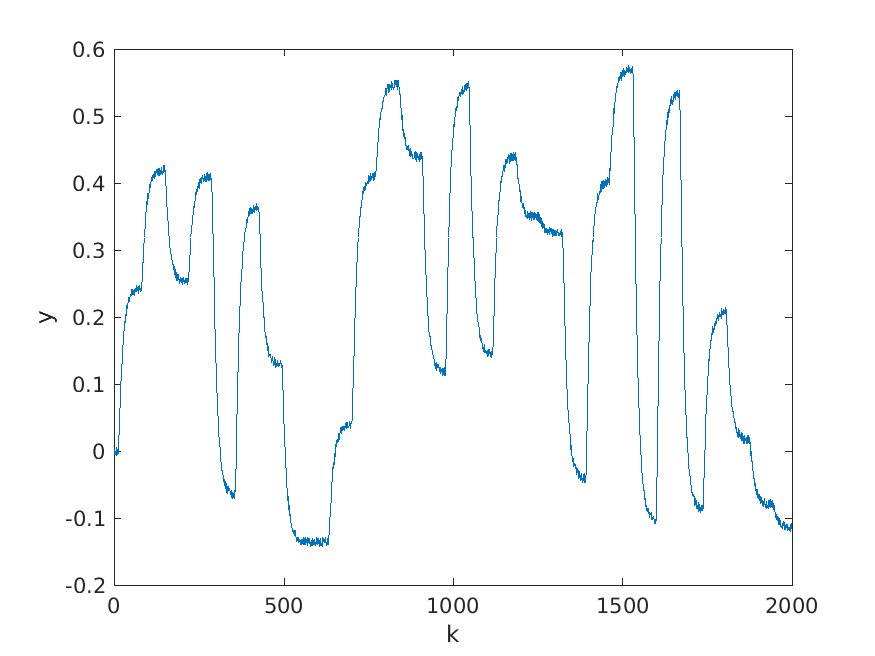
\includegraphics[width=0.7\linewidth]{../dane_dynamiczne/dane_dyn_wer_y}
	\caption{Dane dynamiczne walidujące, wyjście modelu.}
	\label{fig:dane_dyn_wer_y}
\end{figure}

\subsection{Dynamiczne modele liniowe}
Modele postaci $ y(k) = \sum_{i=1}^{n_B}b_i u(k-i) + \sum_{i = 1}^{n_A}a_i y(k-i)$ wyznaczano metodą najmniejszych kwadratów. Wyniki modeli bez rekurencji przedstawia tabela \ref{tab:bez_rek} oraz rysunki \ref{fig:model_bez_rek_train_1}, \ref{fig:model_bez_rek_walid_1}, \ref{fig:model_bez_rek_train_2}, \ref{fig:model_bez_rek_walid_2}, \ref{fig:model_bez_rek_train_3} i \ref{fig:model_bez_rek_walid_3}.
\begin{table}
	\begin{tabular}{|c|c|c|c|c|c|c|c|c|}
		\hline 
		$N$ & $b_3$ & $b_2$ & $b_1$ & $a_3$ & $a_2$ & $a_1$ & $E_{ucz}$ & $E_{wer}$ \\ 
		\hline 
		1 & - & - & 0.0019 & - & - & 0.9989 & 0.1533 & 0.1857 \\ 
		\hline 
		2 & - & -0.0002 & 0.0016 & - & 1.3282 & -0.3294 & 0.1366 & 0.1495 \\ 
		\hline 
		3 & 0.0014 & -0.0002 & -0.0005  & 1.1681  & 0.3155 & -0.4852 & 0.1044 & 0.1130 \\ 
		\hline 
	\end{tabular}
	\label{tab:bez_rek}
	\caption{Modele liniowe bez rekurencji}
\end{table}

\begin{figure}
	\centering
	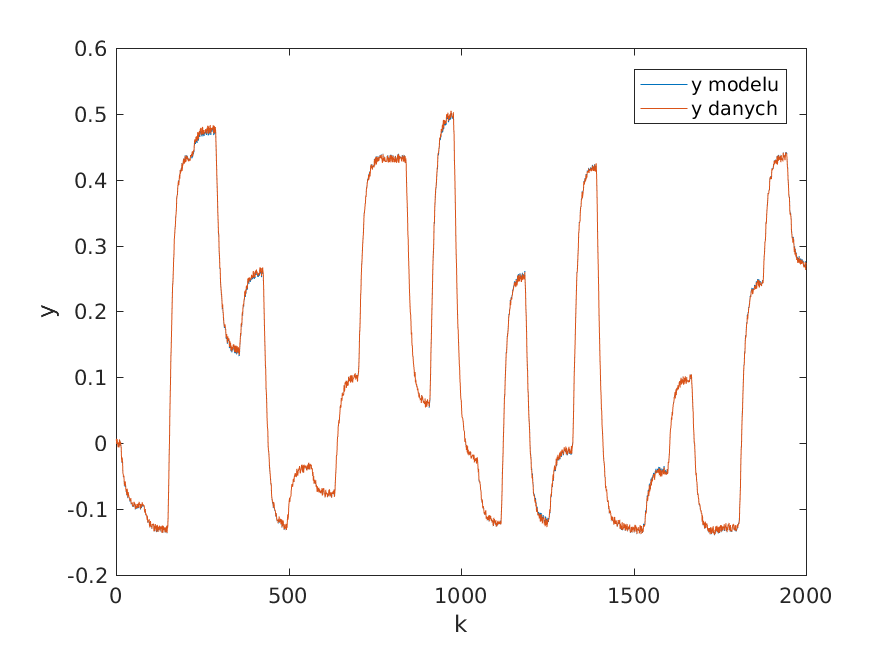
\includegraphics[width=0.7\linewidth]{../dane_dynamiczne/model_bez_rek_train_1}
	\caption{Dane dynamiczne trenujące, na tle modelu pierwszego rzędu bez rekurencji.}
	\label{fig:model_bez_rek_train_1}
\end{figure}

\begin{figure}
	\centering
	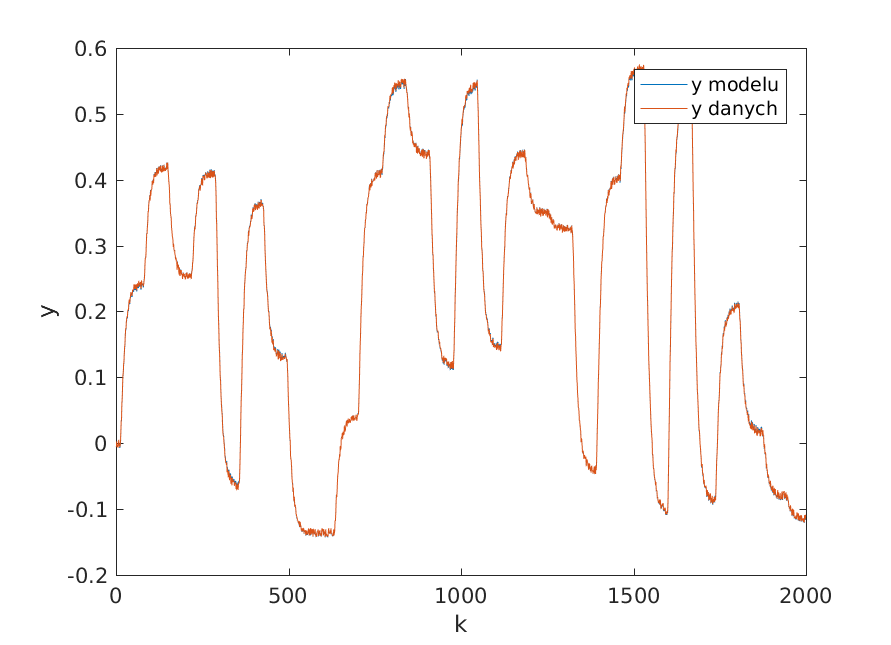
\includegraphics[width=0.7\linewidth]{../dane_dynamiczne/model_bez_rek_walid_1}
	\caption{Dane dynamiczne weryfikacyjne, na tle modelu pierwszego rzędu bez rekurencji.}
	\label{fig:model_bez_rek_walid_1}
\end{figure}

\begin{figure}
	\centering
	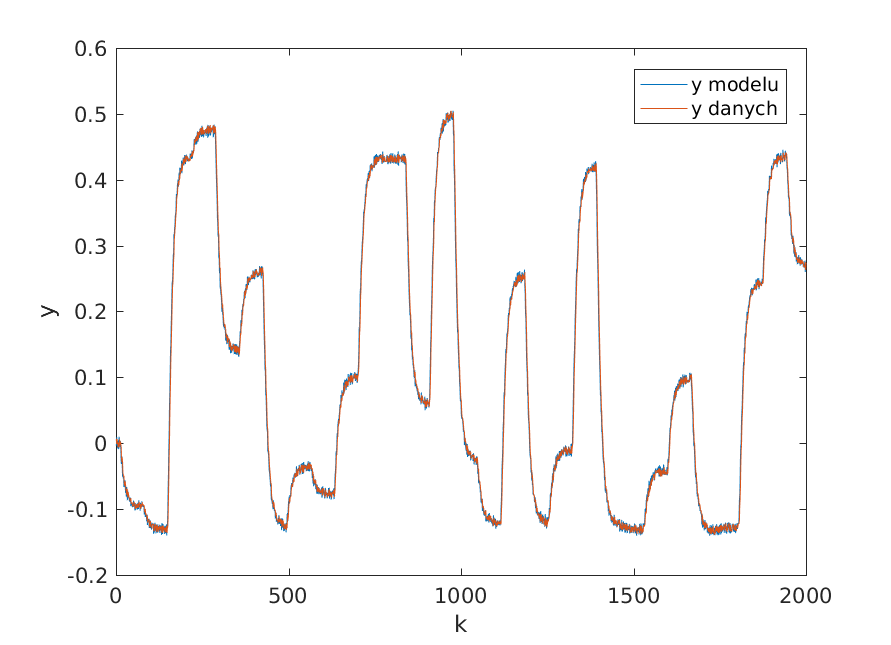
\includegraphics[width=0.7\linewidth]{../dane_dynamiczne/model_bez_rek_train_2}
	\caption{Dane dynamiczne trenujące, na tle modelu drugiego rzędu bez rekurencji.}
	\label{fig:model_bez_rek_train_2}
\end{figure}

\begin{figure}
	\centering
	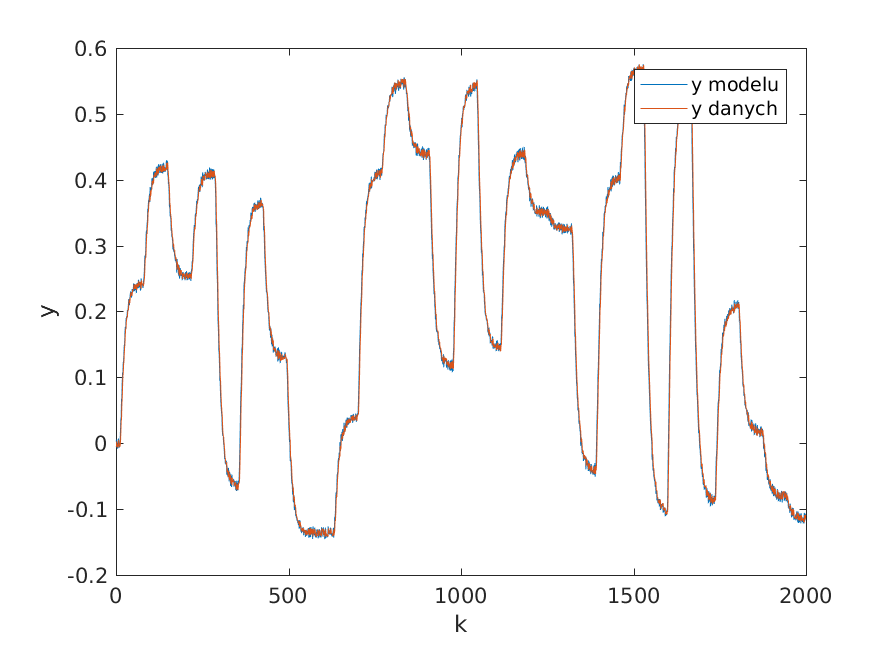
\includegraphics[width=0.7\linewidth]{../dane_dynamiczne/model_bez_rek_walid_2}
	\caption{Dane dynamiczne weryfikacyjne, na tle modelu drugiego rzędu bez rekurencji.}
	\label{fig:model_bez_rek_walid_2}
\end{figure}

\begin{figure}
	\centering
	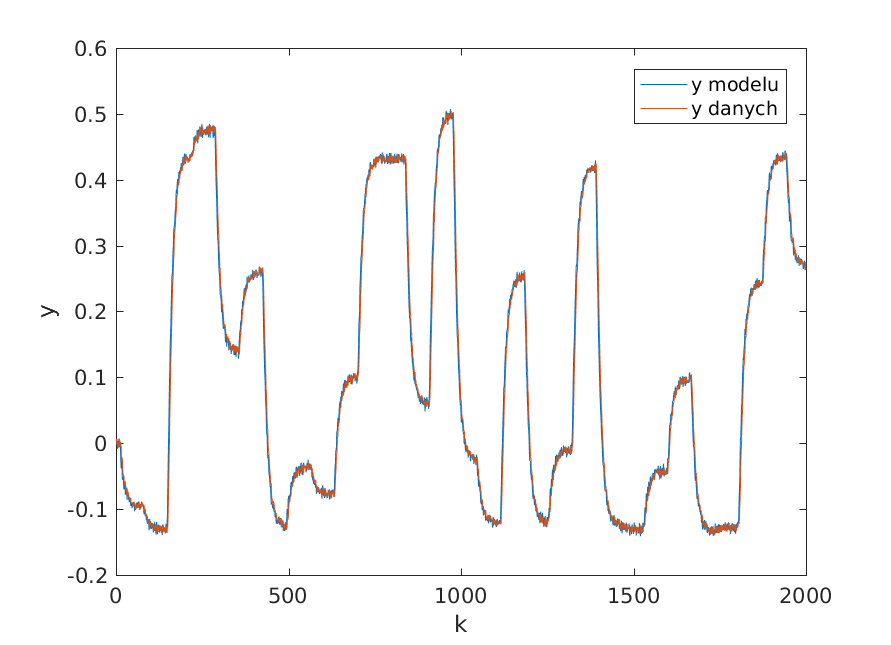
\includegraphics[width=0.7\linewidth]{../dane_dynamiczne/model_bez_rek_train_3}
	\caption{Dane dynamiczne trenujące, na tle modelu trzeciego rzędu bez rekurencji.}
	\label{fig:model_bez_rek_train_3}
\end{figure}

\begin{figure}
	\centering
	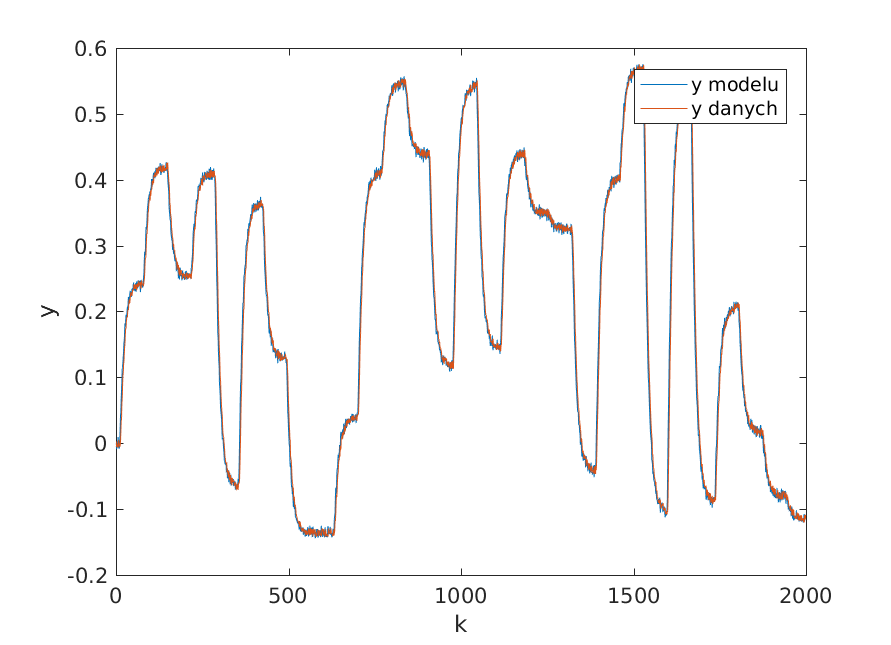
\includegraphics[width=0.7\linewidth]{../dane_dynamiczne/model_bez_rek_walid_3}
	\caption{Dane dynamiczne weryfikacyjne, na tle modelu trzeciego rzędu bez rekurencji.}
	\label{fig:model_bez_rek_walid_3}
\end{figure}

Wyniki modeli z rekurencją przedstawia tabela \ref{tab:rek} oraz rysunki \ref{fig:model_rek_train_1}, \ref{fig:model_rek_walid_1}, \ref{fig:model_rek_train_2}, \ref{fig:model_rek_walid_2}, \ref{fig:model_rek_train_3} i \ref{fig:model_rek_walid_3}.
\begin{table}
	\begin{tabular}{|c|c|c|c|c|c|c|c|c|}
		\hline 
		$N$ & $b_3$ & $b_2$ & $b_1$ & $a_3$ & $a_2$ & $a_1$ & $E_{ucz}$ & $E_{wer}$ \\ 
		\hline 
		1 & - & - & 0.0019 & - & - & 0.9989 & 180.2920 & 285.4301 \\ 
		\hline 
		2 & - & -0.0002 & 0.0016 & - & 1.3282 & -0.3294 & 161.5449 & 250.1680 \\ 
		\hline 
		3 & 0.0014 & -0.0002 & -0.0005  & 1.1681  & 0.3155 & -0.4852 & 123.4280
		 & 196.1376 \\ 
		\hline 
	\end{tabular}
	\label{tab:rek}
	\caption{Modele liniowe z rekurencją}
\end{table}

\begin{figure}
	\centering
	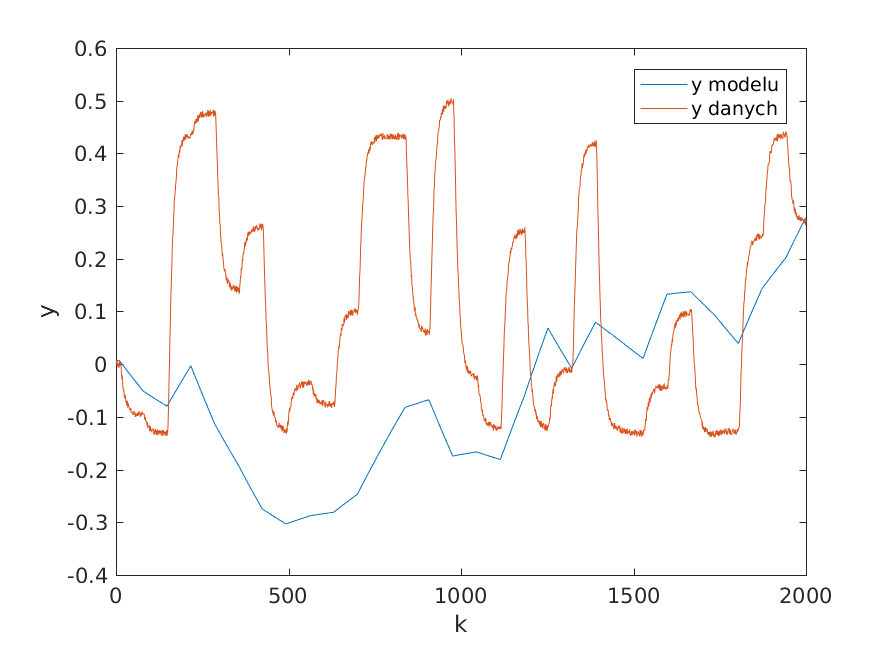
\includegraphics[width=0.7\linewidth]{../dane_dynamiczne/model_rek_train_1}
	\caption{Dane dynamiczne trenujące, na tle modelu pierwszego rzędu z rekurencją.}
	\label{fig:model_rek_train_1}
\end{figure}

\begin{figure}
	\centering
	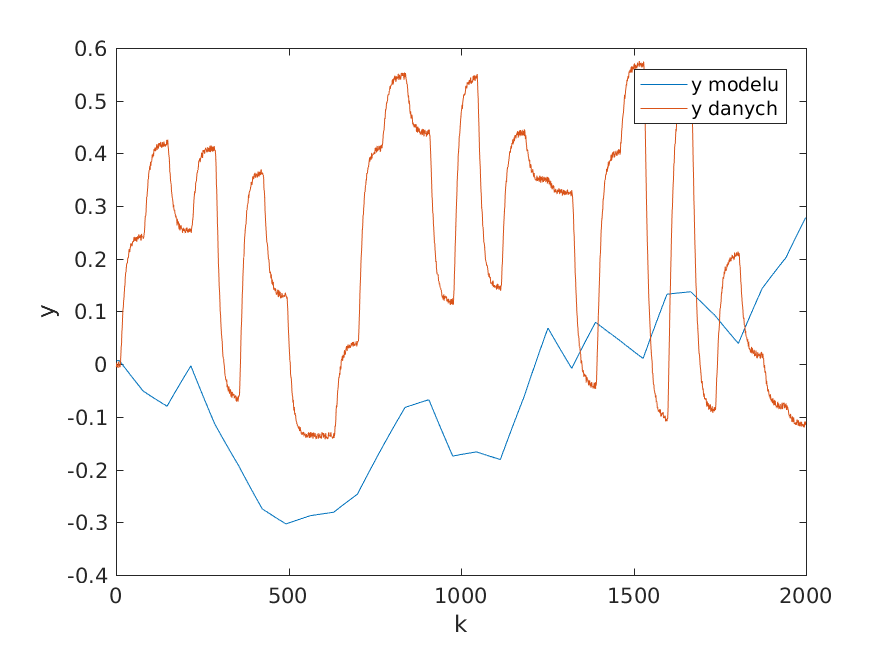
\includegraphics[width=0.7\linewidth]{../dane_dynamiczne/model_rek_walid_1}
	\caption{Dane dynamiczne weryfikacyjne, na tle modelu pierwszego rzędu z rekurencją.}
	\label{fig:model_rek_walid_1}
\end{figure}

\begin{figure}
	\centering
	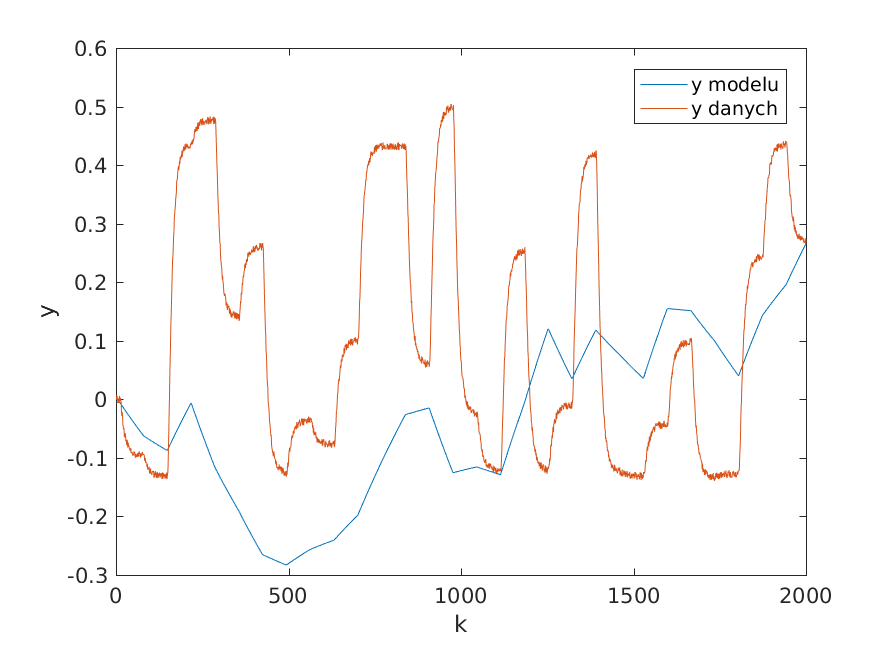
\includegraphics[width=0.7\linewidth]{../dane_dynamiczne/model_rek_train_2}
	\caption{Dane dynamiczne trenujące, na tle modelu drugiego rzędu z rekurencją.}
	\label{fig:model_rek_train_2}
\end{figure}

\begin{figure}
	\centering
	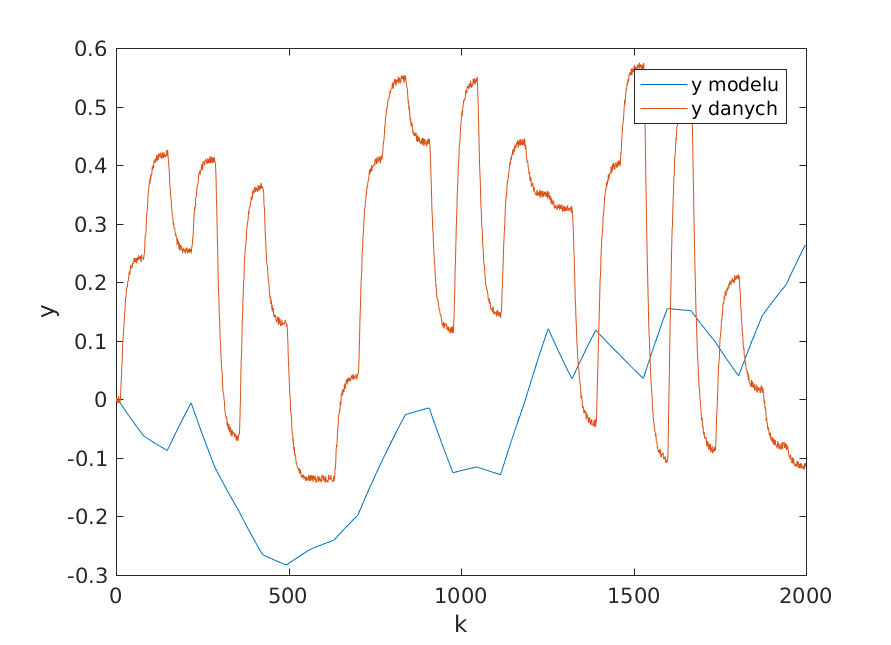
\includegraphics[width=0.7\linewidth]{../dane_dynamiczne/model_rek_walid_2}
	\caption{Dane dynamiczne weryfikacyjne, na tle modelu drugiego rzędu z rekurencją.}
	\label{fig:model_rek_walid_2}
\end{figure}

\begin{figure}
	\centering
	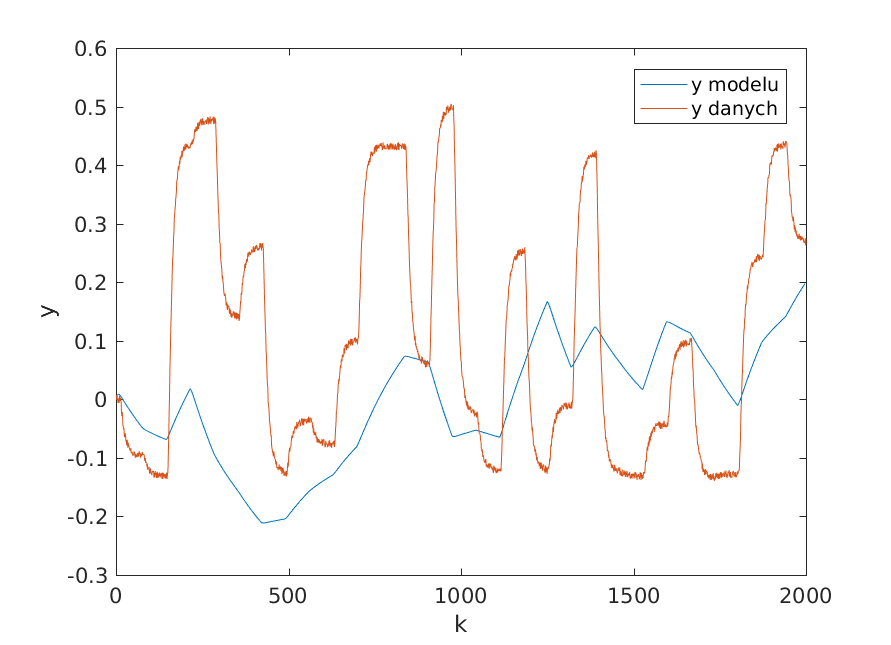
\includegraphics[width=0.7\linewidth]{../dane_dynamiczne/model_rek_train_3}
	\caption{Dane dynamiczne trenujące, na tle modelu trzeciego rzędu z rekurencją.}
	\label{fig:model_rek_train_3}
\end{figure}

\begin{figure}
	\centering
	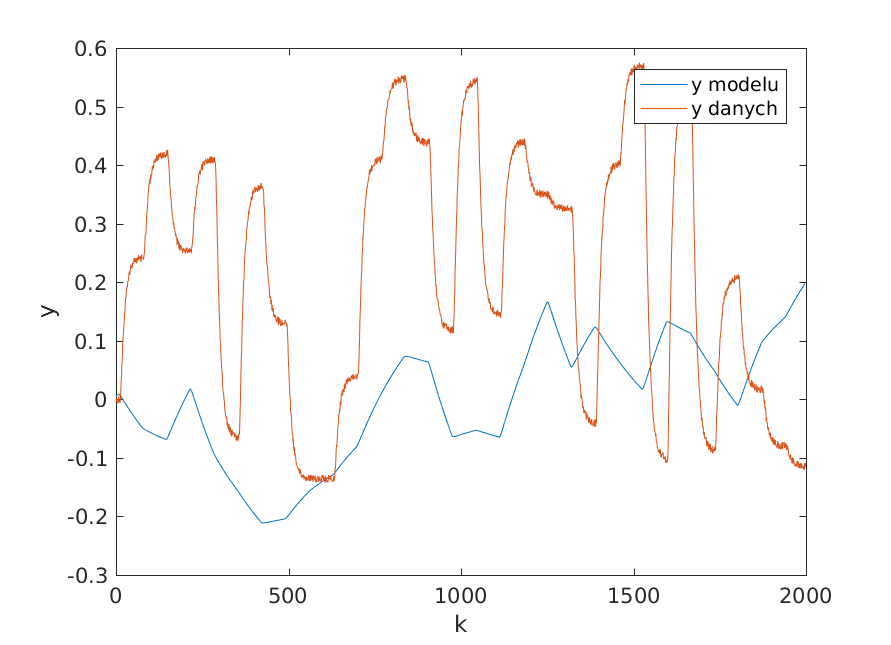
\includegraphics[width=0.7\linewidth]{../dane_dynamiczne/model_rek_walid_3}
	\caption{Dane dynamiczne weryfikacyjne, na tle modelu trzeciego rzędu z rekurencją.}
	\label{fig:model_rek_walid_3}
\end{figure}
Modele bez rekurencji ogólnie działają dobrze (wykresy danych i modeli praktycznie się pokrywają). Najlepszy jest model rzędu trzeciego, lecz prostszy model rzędu pierwszego nie ma wiele większego błędu. Modele rekurencyjne nie działają dobrze, najlepszy z nich jest model rzędu trzeciego.
\end{document}
